\chapter[BOOM Analytics]{BOOM Analytics}
\label{ch:boom}

We decided to begin the BOOM project with an experiment in construction, by implementing a substantial piece of
distributed software in a data-centric, declarative style. Upon review of recent literature on
datacenter infrastructure (e.g.,~\cite{chubby,gfs-sosp,dynamo,mapreduce-osdi}),
we observed that most of the complexity in these systems relates to the
management of various forms of asynchronously-updated state, including sessions,
protocols, and storage. Although quite complex, few of these systems involve intricate, uninterrupted
sequences of computational steps. Hence, we suspected that datacenter
infrastructure might be a good initial litmus test for our hypotheses about building distributed software.

In this paper, we report on our experiences building \emph{\BOOMA,} an
API-compliant reimplementation of the HDFS distributed file system and the
Hadoop MapReduce engine.  We named these two
components \emph{\BOOM-FS} and \emph{\BOOM-MR}, respectively. In writing \BOOMA,
we preserved the Java API ``skin'' of HDFS and Hadoop, but replaced complex
internal state with a set of relations, and replaced key system
logic with code written in a declarative language.
%  Our goal
% with \BOOMA was first to achieve a functional reimplementation of these systems
% (with competitive performance), and then to extend our work by adding advanced
% fault-tolerance and scale features that are typical for cloud computing.

% We decided to put this idea to the test with an experiment in software engineering: implementing a well-known but non-trivial piece of software infrastructure in a data-centric style, and attempting to extend it with advanced fault-tolerance and scale features that are typical for cloud computing.
% We chose Overlog not because we believe it to be inherently the ``right'' choice, but rather because it seemed like a good enough choice to gain experience.  Part of the exercise in this work is to evaluate its strengths and weaknesses, with an eye toward designing a new languge.
 % to see if a language with a very high level, data-centric abstraction could improve our productivity without introducing major computational bottlenecks.  
 % 
 % 
%We set out to convince ourselves of this idea in a realistic setting.
% Choose a language
% As starting points, we considered practical lessons from the success of MapReduce and SQL in harnessing parallelism, even though they are not general-purpose programming languages. We also examined the declarative domain-specific languages that have emerged in an increasing variety of research communities in recent years (Section~\ref{sec:relwork}).  
% %We were attracted to declarative languages -- i.e. languages based in logic -- because they are amenable not only to parallel dataflow implementations a la MapReduce, but also various guarantees via static code analysis.  
% Among the proposals in the literature, the most natural for our purposes seemed to be the Overlog language introduced in the P2 system~\cite{p2:sosp}. 
% Overlog looked promising for our setting: there is pre-existing code
% for network protocol specification, it has been shown to be useful for
% distributed coordination protocols~\cite{paxonp2}, and it offers an
% elegant metaprogramming framework for static analysis, program
% rewriting, and generation of runtime invariant
% checks~\cite{evitaraced}.  
% Choose a target app
% To evaluate the feasibility of \BOOM, 
% For this purpose, we began building {\em \BOOMA}: an API-compliant
% reimplementation of the HDFS distributed filesystem and the Hadoop
% MapReduce engine.\footnote{\BOOM stands for the {\em Berkeley Orders Of Magnitude} project that grew from this effort.  The aim of the \BOOM project is to build orders of magnitude bigger systems in orders of magnitude less code.} We named these two components {\em \BOOM-FS} and
% {\em \BOOM-MR}, respectively. In writing \BOOMA, we preserved the Java
% API ``skin'' of HDFS and Hadoop, but replaced complex internal state
% with a set of relations.  This enabled us to express
% the system logic in a declarative language.

The Hadoop stack appealed to us as a challenge for two reasons.  First, it
exercises the distributed power of a cluster.  Unlike a farm of independent web
service instances, the HDFS and Hadoop code entails coordination of large
numbers of nodes toward common tasks.  Second, Hadoop is missing significant
distributed systems features like availability and scalability of master
nodes. This allowed us to evaluate the difficulty of extending \BOOMA with
complex features not found in the original codebase.

%  This encouraged us to challenge our hypotheses further: not only would we
% try to re-implement a well-understood distributed application in a data-centric
% fashion, but also evaluate how easy it is to extend with complex features that
% had not been attempted in the original codebase.

We implemented \BOOMA using the Overlog logic language, originally developed for
Declarative Networking~\cite{p2:sosp}.  Overlog has been used with some success to
prototype distributed system protocols, notably in a simple prototype of
Paxos~\cite{paxonp2}, a set of Byzantine Fault Tolerance variants~\cite{singh-nsdi}, a suite of distributed file system consistency
protocols~\cite{pads}, and a distributed hash table routing protocol implemented
by our own group~\cite{p2:sosp}.  On the other hand, Overlog had not previously been
used to implement a full-featured distributed system on the scale of Hadoop and
HDFS\@.  One goal of our work on \BOOMA was to evaluate the strengths and
weaknesses of Overlog for system programming in the large, to inform the design of a new declarative
framework for distributed programming.

\subsection{Contributions}
\label{sec:contributions}
This paper describes our experience implementing and evolving \BOOMA, and
running it on Amazon EC2.  We document the effort required to develop \BOOMA in
Overlog, and the way we were able to introduce significant extensions, including
Paxos-supported replicated-master availability, and multi-master
state-partitioned scalability.  We describe the debugging tasks that arose when
programming at this level of abstraction, and our tactics for metaprogramming
Overlog to instrument our distributed system at runtime.

While the outcome of any software experience is bound in part to the specific
programming tools used, there are hopefully more general lessons that can be
extracted.  To that end, we try to separate out (and in some cases critique) the
specifics of Overlog as a declarative language, and the more general lessons of high-level data-centric
programming.  
%The end goal is to evaluate the benefits of data-centric
%programming for cloud infrastructure and applications.  In that regard 
The more
general data-centric aspect of the work is both positive and language-independent: many of the benefits
we describe arise from exposing as much system state as possible via collection
data types, and proceeding from that basis to write simple code to manage those
collections.%   \jmh{Try to weave this throughout, replacing points where we
%   currently talk about Overlog benefits when appropriate.  We should also have a
%   discussion of (a) ``logic vs. simple iterators'' and (b) state management and
%   temporal issues with a ref to the Dedalus TR.}

% As in any software experience paper, much of our discussion is anecdotal,
% supported only ``softly'' by the code artifacts we produced.  However, we also
% attempt to provide some quantitative evidence for the software engineering
% benefits of data-centric distributed programming.  

As we describe each module of \BOOMA, we report the person-hours we spent
implementing it and the size of our implementation in lines of code (comparing
against the relevant feature of Hadoop, if appropriate). These are noisy
metrics, so we are most interested in numbers that transcend the noise terms:
for example, order-of-magnitude reductions in code size.  We also validate that
the performance of \BOOMA is competitive with the original Hadoop codebase.



% Although our focus in this paper is not on improving the performance of Hadoop, we also present performance measurements on EC2 to validate that our approach does not degrade performance relative to the Java codebase used in production.


% We found that while Hadoop's imperative implementation mixes mechanism and
% policy, our declarative approach led to a natural decoupling of the
% two.  
% In turn \BOOMA is significantly more malleable than vanilla Hadoop. 

% This 
% After twelve months of development, \BOOMA performed as well as vanilla Hadoop, and enabled
% us to easily add complex new features including Paxos-supported
% replicated-master availability, and multi-master state-partitioned
% scalability.  
% 
% Our experience implementing \BOOMA in Overlog was gratifying
% both in its relative ease, and in the lessons learned along the way:
% lessons in how to quickly prototype and debug distributed software,
% and in understanding limitations of Overlog that may contribute to an
% even better programming environment for datacenter development.

%Our principle hypothesis is that recasting the problem of programming 
%distributed systems from a model of explicit communicating processes
%to a 
% Raising the level of abstraction to parallel data manipulation eases the burden of understanding,
% constructing, and evolving such systems.  This assertion is necessarily subjective, 
% and we validate it as best we can.   We consider the reduced complexity of the
% final product through measures like lines of code, the ease of system extensibility
% by illustrating the relative independence and isolation of various modificatons, 
% and the viability of our approach for production systems through performance evaluations.


We present the evolution of \BOOMA from a straightforward reimplementation of
HDFS and Hadoop to a significantly enhanced system.  We describe how our initial
\BOOM-FS prototype went through a series of major revisions (``revs'') focused
on \emph{availability} (Section~\ref{sec:rely}), \emph{scalability}
(Section~\ref{sec:scale}), and \emph{debugging and monitoring}
(Section~\ref{sec:manage}). We then detail how we designed \BOOM-MR by replacing
Hadoop's task scheduling logic with a declarative scheduling framework
(Section~\ref{sec:mr}). In each case, we discuss how the
data-centric approach influenced our design, and how the modifications involved
interacted with earlier revisions.  We compare the performance of \BOOMA with
Hadoop in Section~\ref{sec:eval}, and reflect on the experiment in
Section~\ref{sec:lessons}.

\subsection{Related Work}
\label{sec:relwork}
Declarative and data-centric languages have traditionally been considered useful
in very few domains, but things have changed substantially in recent years.
MapReduce~\cite{mapreduce-osdi} has popularized functional dataflow programming
with new audiences in computing.  Also, a surprising breadth of recent research
projects have proposed and prototyped declarative languages, including overlay
networks~\cite{p2:sosp}, three-tier web services~\cite{hilda}, natural language
processing~\cite{dyna}, modular robotics~\cite{meld}, video
games~\cite{cornellgames}, file system metadata analysis~\cite{wiscfsck}, and
compiler analysis~\cite{bddbddb}.

Most of the languages cited above are declarative in the same sense as SQL: they are based in first-order logic.
 % and specify ``what'' the program outcomes should be, rather than ``how'' to achieve them.  
Some --- notably MapReduce, but also SGL~\cite{cornellgames} --- are
algebraic or dataflow languages, used to describe the
composition of operators that produce and consume sets
or streams of data.  Although arguably imperative, they are far closer
to logic languages than to traditional imperative languages like Java
or C, and are often amenable to set-oriented optimization techniques developed for declarative languages~\cite{cornellgames}.
% . Often there is an equivalence between algebraic and declarative languages; the proof of this equivalence for relational databases helped kick off that field~\cite{Codd72}. Because of these equivalences, declarative optimization techniques and formal proof techniques can be used on algebraic dataflow languages with appropriate hooks
Declarative and dataflow languages can also share the same runtime, as
demonstrated by recent integrations of MapReduce and SQL
in Hive~\cite{hive}, DryadLINQ~\cite{DryadLINQ},
HadoopDB~\cite{hadoopdb}, and products from vendors such as Greenplum and Aster.
% and commercial integrations of SQL and MapReduce.
% ~\cite{greenplum,aster}.
  % By contrast, traditional programming languages ask programmers to focus mostly on imperative threads of control specifying sequences of instructions, which typically run on a single machine and communicate with other threads via shared channels.

%Erlang is an interesting alternative approach to cluster programming.  
Concurrent with our work, the Erlang language was used to implement a simple MapReduce framework called Disco~\cite{disco} and a transactional DHT called Scalaris with Paxos support~\cite{scalaris}.
Philosophically, Erlang revolves around concurrent {\em actors}, rather than
data.  Experience papers regarding Erlang can be found in the literature (e.g.,~\cite{armistice}), and this paper can be seen as a complementary experience paper on building distributed systems in a data-centric fashion.  A closer comparison of actor-oriented and data-centric design styles is beyond the scope of this paper, but an interesting topic for future work.

%: Erlang programmers engage in the specification of small agents that pass messages, and Erlang advocates speak of the high numbers of concurrent ``processes'' involved in an implementation.  
%By contrast, the logic languages described above focus on data, and the logical implications of invariants over that data.  Overlog extends that data-centric notion with implicit asynchronous communication in a simple way.  
%We do not have experience to share regarding the suitability of Erlang for datacenter programming.  
% The Disco FAQ warns that ``Hadoop is probably faster, more scalable, and more featureful''~\cite{disco}.  By contrast, \BOOMA performs as well as Hadoop in apples-to-apples performance tests, and adds significant features.  Overlog seems to offer only modestly more compact code than Erlang --- as one example, the Scalaris Paxos implementation in Erlang has significantly more lines of code than our Overlog version, but in the same order of magnitude.

%\jmh{We need to check that this is not in Disco.  They have partitioned master nodes, it seems, but not fault-tolerant master nodes.}
% , which may not be as natural in Erlang's process-centric model.

Distributed state machines are the traditional formal model for distributed system implementations, and can be expressed in languages like Input/Output Automata (IOA) and the Temporal Logic of Actions (TLA)~\cite{lynchbook}.  By contrast, our approach is grounded in Datalog and its extensions.  % The pros and
% cons of starting with a data-centric foundation are a recurring theme of
% this paper.
% These ideas have been used extensively for network protocol design and verification~\cite{lotos,estelle}.   They also form the basis of the MACE~\cite{mace} language for overlay networks.  
%Those languages do not offer the query-like facilities for monitoring and management that data-centric languages provide, which we exploit for manageability and debugging as described in Section~\ref{sec:manage}. 
%These facilities seemed particularly useful for protocols such as Paxos that were originally specified in terms of logical invariants. %\rcs{Joe we changed this; we think sets of invariants are a better approach than IOA, TLA, and state machines are an artifact of existing languages}  
%As we discuss in Section~\ref{sec:manage}, this was confirmed by our experience, especially when we were able to convince ourselves of the correctness of our implementations by metaprogramming our logic.

Our use of metaprogrammed Overlog was heavily influenced by the Evita Raced
Overlog metacompiler~\cite{evitaraced}, and the security and typechecking
features of Logic Blox' LBTrust~\cite{lbtrust}.  Some of our monitoring tools
were inspired by Singh et al.~\cite{singh-eurosys}, although our metaprogrammed
implementation avoids the need to modify the language runtime as was done in that work.

ubsection{JOL}
The original Overlog implementation (\emph{P2}) is aging and targeted at network
protocols, so we developed a new Java-based Overlog runtime we call \emph{\JOL.}
Like P2, \JOL compiles Overlog programs into pipelined dataflow graphs of
operators (similar to ``elements'' in the Click modular router~\cite{click}).
\JOL provides \emph{metaprogramming} support akin to P2's Evita Raced
extension~\cite{evitaraced}: each Overlog program is compiled into a
representation that is captured in rows of tables.  Program testing,
optimization and rewriting can be written concisely as metaprograms in Overlog
that manipulate those tables.

Because the Hadoop stack is implemented in Java, we anticipated the need for
tight integration between Overlog and Java code. Hence, \JOL supports Java-based
extensibility in the model of Postgres~\cite{postgres}.  It supports Java
classes as abstract data types, allowing Java objects to be stored in fields of
tuples, and Java methods to be invoked on those fields from Overlog.  \JOL also
allows Java-based aggregation functions to run on sets of column values, and
supports Java \emph{table functions}: Java iterators producing tuples, which can
be referenced in Overlog rules as ordinary relations. We made significant use of
each of these features in \BOOMA.

%In addition, inspired by the ideas of Evita Raced, we metaprogrammed \JOL's core execution loop and scheduler in Overlog as well.  Rather than using a traditional event loop,  in \JOL all inbound events (i.e., tuples) are passed into a single dataflow compiled from the system's runtime metaprogram. This dataflow ``routes'' tuples to appropriate branches corresponding to different rules, using a scheduler specified in Overlog.  Space prevents a thorough discussion of this design, but we mention it here because of our experience modifying the runtime rules as described in Section~\ref{sec:perf}.  

\section{MapReduce Port}
\label{sec:mr}
In contrast to our clean-slate strategy for developing \BOOM-FS, we built
\BOOM-MR, our MapReduce implementation, by replacing Hadoop's core scheduling
logic with Overlog. Our goal in building \BOOM-MR was to explore embedding a
data-centric rewrite of a non-trivial component into an existing procedural
system.  MapReduce scheduling policies are one issue that has been treated in
recent literature (e.g.,~\cite{late-sched,delay-sched}).  To enable credible
work on MapReduce scheduling, we wanted to remain true to the basic structure of
the Hadoop MapReduce codebase, so we proceeded by understanding that code,
mapping its core state into a relational representation, and then writing
Overlog rules to manage that state in the face of new messages delivered by the
existing Java APIs.  We follow that structure in our discussion.

\subsection{Background: Hadoop MapReduce}
In Hadoop MapReduce, there is a single master node called the \emph{\JT} which
manages a number of worker nodes called \emph{{\TT}s}.  A job is divided into a
set of map and reduce \emph{tasks}. The {\JT} assigns tasks to worker nodes.  Each
map task reads an input chunk from the distributed file system, runs a
user-defined map function, and partitions output key/value pairs into hash
buckets on the local disk.  Reduce tasks are created for each hash
bucket.  Each reduce task fetches the corresponding hash buckets from all
mappers, sorts locally by key, runs a user-defined reduce function and writes
the results to the distributed file system.

Each {\TT} has a fixed number of slots for executing tasks (two maps and two
reduces by default). A heartbeat protocol between each {\TT} and the {\JT} is
used to update the {\JT}'s bookkeeping of the state of running tasks, and drive
the scheduling of new tasks: if the {\JT} identifies free {\TT} slots, it will
schedule further tasks on the {\TT}. Also, Hadoop will attempt to schedule
\emph{speculative} tasks to reduce a job's response time if it detects
``straggler'' nodes~\cite{mapreduce-osdi}.

\subsection{MapReduce Scheduling in Overlog}
\label{sec:mr-overlog}
Our initial goal was to port the {\JT} code to Overlog.  We began by identifying
the key state maintained by the {\JT}.  This state includes both data structures
to track the ongoing status of the system and transient state in the form of
messages sent and received by the {\JT}.  We captured this information in four
Overlog tables, shown in Table~\ref{tbl:hcatalog}.

\begin{table}
\centering
\scriptsize{
\begin{tabular}{|l|l|l|} \hline
\textit{Name}   & \textit{Description} & \textit{Relevant attributes} \\ \hline\hline
job          & Job definitions   & \underline{jobid}, priority, submit\_time, \\ 
             &                   & status, jobConf \\ \hline
task         & Task definitions  & \underline{jobid}, \underline{taskid}, type, partition, status \\ \hline
taskAttempt  & Task attempts      & \underline{jobid}, \underline{taskid}, \underline{attemptid}, progress, \\
             &       & state, phase, tracker, input\_loc, \\ 
             &       & start, finish \\ \hline
taskTracker  & {\TT}             & \underline{name}, hostname, state, \\
             & definitions       & map\_count, reduce\_count, \\
             &                   & max\_map, max\_reduce\\ \hline
\end{tabular}
}
\caption{\BOOM-MR relations defining {\JT} state.}
\vspace{-8pt}
\label{tbl:hcatalog}
\end{table}

The \emph{job} relation contains a single row for each job submitted to the
{\JT}. In addition to some basic metadata, each job tuple contains an attribute
called \emph{jobConf} that holds a Java object constructed by legacy Hadoop
code, which captures the configuration of the job. The \emph{task} relation
identifies each task within a job. The attributes of this relation identify the
task type (map or reduce), the input ``partition'' (a chunk for map tasks, a
bucket for reduce tasks), and the current running status.

A task may be attempted more than once, due to speculation or if the initial
execution attempt failed.  The \emph{taskAttempt} relation maintains the state
of each such attempt.  In addition to a progress percentage and a state
(running/completed), reduce tasks can be in any of three phases: copy, sort, or
reduce. The \emph{tracker} attribute identifies the {\TT} that is assigned to
execute the task attempt. Map tasks also need to record the location of their
input data, which is given by \emph{input\_loc}. The \emph{taskTracker} relation
identifies each {\TT} in the cluster with a unique name.

%It is also used to constrain the scheduler, which can assign map and reduce tasks up to the max\_map and max\_reduce attributes of each tracker. %\jmh{drop dirty?}
%The hostname, current running state, and task workload of the \TT are also part of this relation. 
%The map\_count and reduce\_count attributes indicate how many map and reduce tasks are currently running on the \TT. The maximum number of map and reduce tasks that the \TT is able to support are given by the max\_map and max\_reduce attributes; this is in keeping with Hadoop which specifies these values in each message from a \TT to the \JT.

%Having ``table-ized'' the \JT internals, we still had to translate from the traditional Java-based Hadoop APIs into this representation.  For inbound messages, we stubbed out the original Java message handlers to place tuples on the \JOL event queue, where they are picked up by the \JOL runtime. We chose to leave Hadoop's job configuration parsing untouched; it populates the jobConf field of the {\em job} table. We wrote our Overlog rules to place outbound messages into the {\em trackerAction} table of Table~\ref{tbl:hcatalog}.  We then modified Hadoop's Java heartbeat code to drain this table via a simple \JOL call between timesteps, and send the corresponding API action to the \TT mentioned in each {\em trackerAction} tuple.  \jmh{Isn't this out-of-date?  I.e. we don't invoke Hadoop API calls to talk to the TaskTracker anymore.}


Overlog rules are used to update the {\JT}'s tables by converting inbound messages
into \emph{job}, \emph{taskAttempt} and \emph{taskTracker} tuples. These rules
are mostly straightforward. Scheduling decisions are encoded in the
\emph{taskAttempt} table, which assigns tasks to {\TT}s. A scheduling policy is
simply a set of rules that join against the \emph{taskTracker} relation to find
\TT{}s with unassigned slots, and schedules tasks by inserting tuples into
\emph{taskAttempt}. This architecture makes it easy for new scheduling policies
to be defined.

%%\begin{table}[h]
%%\centering
%%\scriptsize{
%%\begin{tabular}{|l|r|r|} \hline
%%{\it System}   & {\it Lines in Patch} & {\it Files Modified by Patch} \\ \hline\hline
%%Hadoop       & 2102   & 17 \\ \hline
%%\BOOM-MR & 82    & 2 \\ \hline
%%\end{tabular}
%%}
%%\caption{Modifying MapReduce schedulers with LATE.\vspace{-12pt}}
%%\vspace{-10pt}
%%\label{tbl:latepatch}
%%\end{table}

% To exercise our extensible scheduling architecture, we implemented the LATE
% scheduler~\cite{late-sched}, in addition to Hadoop's default
% scheduling policy.  
% The LATE policy is specified in the paper via just three lines of
% pseudocode, which the authors of that paper translated into an 800 line Java code patch. In comparison,
% we were able to express LATE using only 5 additional Overlog rules that can be
% applied to the scheduler through a 30 line code patch. Further details of our LATE implementation
% can be found in~\cite{boom-techr}.

%%Table~\ref{tbl:latepatch} quantifies the relative complexity of the Java
%%LATE scheduler patch against Hadoop (\cite{jira}, issue HADOOP-2141)
%%with the size of our LATE implementation in \BOOM-MR.  Appendix~\ref{sec:scheduling} 
%%validates the faithfulness of our implementation in practice.  In sum, we were pleased
%%to see that the \BOOM approach enabled scheduler modifications that were over an order of magnitude
%%smaller than traditional approaches.

%; for space reasons, we defer discussion of our LATE implementation to Appendix~\ref{sec:scheduling}.

% \subsubsection{\JT Logic}
% The core of the \JT logic was captured in three basic sets of rules: job and task bookkeeping, %\jmh{(jobtracker.olg)}, 
% a scheduling harness,
% % \jmh{(scheduler.olg)} 
% and pluggable scheduling policies.
% % \jmh{(policy.olg)}. 
%P2 showed how asynchronous messaging can be compactly represented via rules that join an incoming message stream with tables representing dispatching policies and local state updates. The Overlog execution loop reviewed in Section~\ref{sec:jol} atomically handles snapshotting the incoming stream of messages as a Datalog table, deducing the effects of all handlers, applying the results to local state, and generating response messages as appropriate.  
%Each \TT message is translated into one {\em TaskTracker} tuple and zero or more {\em TaskAttempt} tuples, which \JOL uses to update the corresponding tables before the next fixpoint computation.
%As we discuss in Section~\ref{sec:manage}, we had to revisit our initial prototype later, to pare down the logic captured in each handler.

%jobtracker.olg
% The bookkeeping module maintains the state of jobs and tasks. Hadoop receives job requests via XML job configuration files.  It constructs a jobConf object from each such file, and our stub code then generates a {\em job} table tuple containing that jobConf object which it places on the \JOL event queue.  \JOL inserts that tuple into the {\em job} table.  During the fixpoint computation, an Overlog rule generates {\em task} tuples from that {\em job} tuple -- one for each map and reduce task that make up the job. Hadoop also receives heartbeats from {\TT}s; these are converted to {\em taskAttempt} tuples and placed on the \JOL event queue.
% Task state is derived by a query that identifies the taskAttempt tuple with the maximum progress for each task. The job status is maintained by another aggregation query over the task relation that combines the state of each task that is part of the job. 
% 
% %\jmh{finish me... be sure that this paragraph coupled with the last one explains how the system event loop ``ticks''.}
% The scheduling harness is made up of two modules. The scheduler.olg module translates updates to the taskTracker relation into scheduling units of work (slots). A tracker periodically updates its map\_count and reduce\_count values in the taskTracker relation.  The difference between these counts and the maximum map and reduce counts in the taskTracker relation indicates the amount of new work we can schedule on the {\TT}.  The value is sent to the policy.olg module in the form of map and reduce slot counts, which initiates a set of queries that determine what task(s) it should schedule on the tracker. These tasks are picked up by the scheduler.olg module, and are translated into launch task actions on the \TT.
% 
% The jobtracker and scheduler modules are periodically executed by the system. The jobtracker.olg module executes by performing a lookup over the taskAttempt relation for attempt rows that have been updated by {\TT}ers. An update to a task attempt is indicated by the dirty attribute of the taskAttempt relation. An index is defined on the dirty attribute in order to avoid a full can of this relation. The scheduler.olg module executes by performing a lookup over the taskTracker relation for updated rows (again indicated by a dirty attribute). 
% 
% Scheduling policies were simply encapsulated as rules that \jmh{finish me...}.
% 
% \jmh{Conclude with what was hard what was easy (line counts, 
% including java added/deleted and overlog written).
% Reflect on the OverLog to Java boundary? }\rcs{ I will have things to say about the BFS Overlog/java boundary below...  do we want to split up the discussion of such things?}

\subsection{Evaluation}
\label{sec:schedeval}
To validate the extensible scheduling architecture described in
Section~\ref{sec:mr-overlog}, we implemented both Hadoop's default
First-Come-First-Serve (FCFS) policy and the LATE policy proposed by Zaharia et
al.~\cite{late-sched}. Our goals were both to evaluate the difficulty of
building a new policy, and to confirm the faithfulness of our Overlog-based
{\JT} to the Hadoop {\JT} using two different scheduling algorithms.

Implementing the default FCFS policy required 9 rules (96 lines of
code). Implementing the LATE policy required 5 additional Overlog rules (30
lines of code). In comparison, LATE is specified in Zaharia et al.'s paper via
just three lines of pseudocode, but their implementation of the policy for
vanilla Hadoop required adding or modifying over 800 lines of Java --- an order
of magnitude more than our Overlog implementation. Further details of our LATE
implementation can be found in the technical report~\cite{boom-techr}.

We now compare the behavior of our LATE implementation with the results observed
by Zaharia et al.\ using Hadoop MapReduce. We used a 101-node cluster on Amazon
EC2. One node executed the Hadoop \JT\ and the HDFS \NN, while the remaining 100
nodes served as slaves for running the Hadoop {\TT}s and HDFS {\DN}s. Each {\TT}
was configured to support executing up to two map tasks and two reduce tasks
simultaneously. The master node ran on a ``high-CPU extra large'' EC2 instance
with 7.2 GB of memory and 8 virtual cores. Our slave nodes executed on
``high-CPU medium'' EC2 instances with 1.7 GB of memory and 2 virtual
cores. Each virtual core is the equivalent of a 2007-era 2.5Ghz Intel Xeon
processor.

LATE focuses on how to improve job completion time by reducing the impact of
``straggler'' tasks. To simulate stragglers, we artificially placed additional
load on six nodes. We ran a wordcount job on 30 GB of data, using 481 map tasks
and 400 reduce tasks (which produced two distinct ``waves'' of reduces). We ran
each experiment five times, and report the average over all
runs. Figure~\ref{fig:ec2reduce} shows the reduce task duration CDF for three
different configurations. The plot labeled ``No Stragglers'' represents normal
load, while the ``Stragglers'' and ``Stragglers (LATE)'' plots describe
performance in the presence in stragglers using the default FCFS policy and the
LATE policy, respectively. We omit map task durations, because adding artificial
load had little effect on map task execution --- it just resulted in slightly
slower growth from just below 100\% to completion.

The first wave of 200 reduce tasks was scheduled at the beginning of the
job. This first wave of reduce tasks cannot finish until all map tasks have
completed, which increased the duration of these tasks as indicated in the right
portion of the graph. The second wave of 200 reduce tasks did not experience
delay due to unfinished map work since it was scheduled after all map tasks had
finished. These shorter task durations are reported in the left portion of the
graph. Furthermore, stragglers had less impact on the second wave of reduce
tasks since less work (i.e., no map work) is being
performed. Figure~\ref{fig:ec2reduce} shows this effect, and also demonstrates
how the LATE implementation in {\BOOMA} handles stragglers much more effectively
than the FCFS policy ported from Hadoop.  This echoes the results of Zaharia et
al.~\cite{late-sched}

\begin{figure}
  \centering
  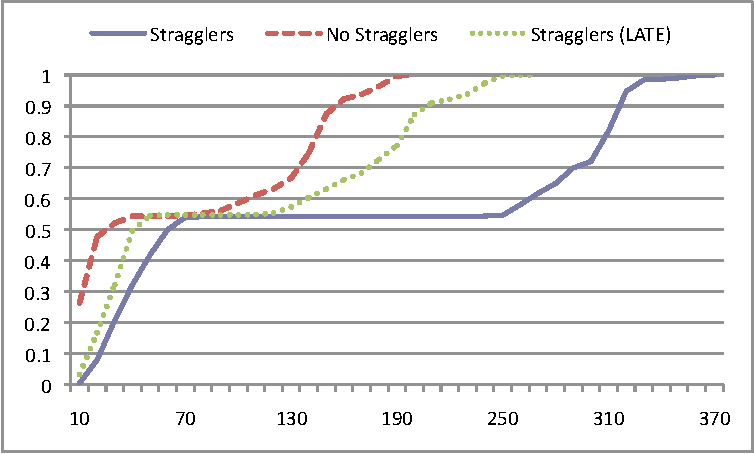
\includegraphics{figures/reduce_stragglers}
  \caption{CDF of reduce task duration (secs), with and without stragglers.}
  \label{fig:ec2reduce}
\end{figure}

\subsection{Discussion}
The initial version of \BOOM-MR required one person-month of
development time. We spent an additional two person-months debugging
and tuning \BOOM-MR's performance for large jobs. \BOOM-MR consists of
55 Overlog rules in 396 lines of code, and 1269 lines of Java.
\BOOM-MR is based on Hadoop version 18.1; we estimate that we removed
6,573 lines from Hadoop (out of 88,864). The removed code contained
the core scheduling logic and the data structures that represent the
components listed in Table~\ref{tbl:hcatalog}. The Overlog patch that
replaces the original Hadoop scheduler contains an order of magnitude
fewer lines of code.  The performance of \BOOM-MR is very similar to
that of Hadoop MapReduce, as we discuss in Section~\ref{sec:eval}.

%% Our experience gutting Hadoop and inserting \BOOMA was not always
%% pleasant.  Given that we were committed to preserving the client API,
%% we did not take a ``purist'' approach and try to convert everything
%% into tables and Overlog rules.  For example, we chose not to
%% ``tableize'' the JobConf object, but instead to carry it through
%% Overlog tuples.  In our Overlog rules, we pass the JobConf object into
%% a custom Java table function that manufactures {\em task} tuples for
%% the job, subject to the specifications in the JobConf.

For this ``porting'' exercise, it was handy to leverage \JOL's Java interfaces
and draw the Java/Overlog boundaries flexibly.  This allowed us to focus on
porting the more interesting Hadoop logic into Overlog, while avoiding ports of
relatively mechanical details.  For example, we chose to leave the data
representation of the \emph{jobConf} as a Java object rather than flatten it
into a relation because it had no effect on the scheduling logic.

We found that scheduling policies were a good fit for a declarative language
like Overlog. In retrospect, this is because scheduling can be decomposed into
two tasks: \emph{monitoring} the state of a system and applying \emph{policies}
for how to react to changes to that state. Monitoring is well-handled by
Overlog: we found that the statistics about {\TT} state required by the LATE
policy are naturally realized as aggregate functions, and \JOL took care of
automatically updating those statistics as new messages from {\TT}s arrived. It
is also unsurprisingly that a logic language should be well-suited to specifying
policy. Overall, we found the \BOOM-MR scheduler much simpler to extend and
modify than the original Hadoop Java code, as demonstrated by our experience
with LATE\@.  Informally, the Overlog code in \BOOM-MR seems about as complex as
it should be: Hadoop's MapReduce task coordination logic is a simple and clean
design, and the compactness of \BOOM-MR reflects that simplicity appropriately.


\begin{figure}
	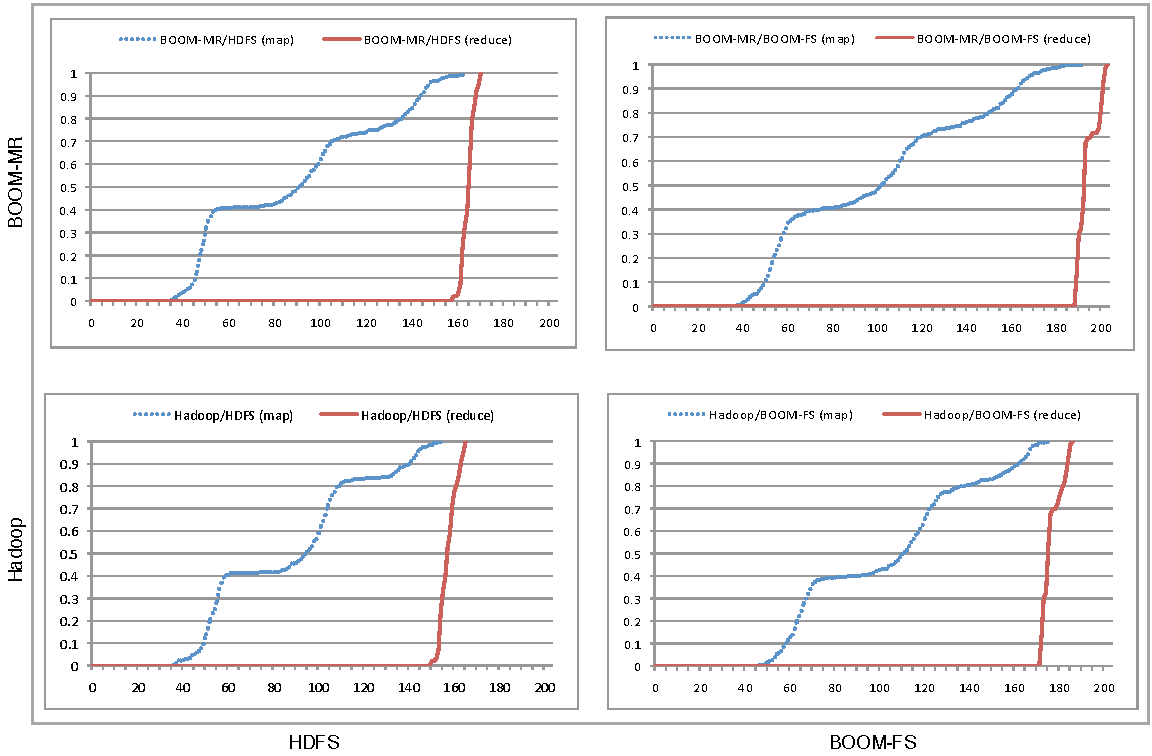
\includegraphics{figures/fourgraphs}
\caption{CDFs representing the elapsed time between job startup and task
  completion for both map and reduce tasks, for all combinations of Hadoop and \BOOM-MR
  over HDFS and \BOOM-FS\@.  In each graph, the horizontal axis is
  elapsed time in seconds, and the vertical represents the percentage of tasks completed.}
\label{fig:ec2experiment}
\end{figure}

\section{Performance Validation}
\label{sec:eval}
While improved performance was not a goal of our work, we wanted to
ensure that the performance of \BOOMA was competitive with Hadoop.
We compared \BOOMA with Hadoop 18.1, using the 101-node EC2 cluster
described in Section~\ref{sec:schedeval}. The workload was a wordcount job
on a 30 GB file, using 481 map tasks and 100 reduce tasks.

Figure~\ref{fig:ec2experiment} contains four graphs comparing the performance of
different combinations of Hadoop MapReduce, HDFS, \BOOM-MR, and \BOOM-FS\@. Each
graph reports a cumulative distribution of the elapsed time in seconds from job
startup to map or reduce task completion. The map tasks complete in three
distinct ``waves.'' This is because only 2 $\times$ 100 map tasks can be
scheduled at once. Although all 100 reduce tasks can be scheduled immediately,
no reduce task can finish until all maps have been completed because each reduce
task requires the output of all map tasks.

The lower-left graph describes the performance of Hadoop running on top of HDFS,
and hence serves as a baseline for the subsequent graphs. The upper-left graph
details \BOOM-MR running over HDFS\@. This graph shows that map and reduce task
durations under \BOOM-MR are nearly identical to Hadoop 18.1. The lower-right
and upper-right graphs detail the performance of Hadoop MapReduce and \BOOM-MR
running on top of \BOOM-FS, respectively. \BOOM-FS performance is slightly
slower than HDFS, but remains competitive.

% The LATE policy presents an alternative scheme for speculative task
% execution on {\em straggler} tasks~\cite{late-sched}, in an effort to
% improve on Hadoop's policy.  There are two aspects to each policy:
% choosing which tasks to speculatively re-execute, and choosing {\TT}s
% to run those tasks.  Original Hadoop re-executes a task if its
% progress is more than 0.2 (on a scale of $[0..1]$) below the mean
% progress of similar tasks; it assigns speculative tasks using the same
% policy as it uses for initial tasks. LATE chooses tasks to re-execute
% via an {\em estimated finish time} metric based on the task's
% \emph{progress rate}. Moreover, it avoids assigning speculative tasks
% to {\TT}s that exhibit slow performance executing similar tasks, in
% hopes of preventing the creation of new stragglers.

%%The LATE policy is specified in the paper via just three lines of
%%pseudocode, which make use of three performance statistics called {\em
%%  SlowNodeThreshold}, {\em SlowTaskThreshold}, and {\em
%%  SpeculativeCap}.  The first two of these statistics correspond to
%%the 25th percentiles of progress rates across {\TT}s and across tasks,
%%respectively.  The {\em SpeculativeCap} is suggested to be set at 10\%
%%of available task slots~\cite{late-sched}.  We compute these
%%thresholds via the five Overlog rules shown in
%%Figure~\ref{fig:latePolicy}.  Integrating the rules into \BOOM-MR
%%required modifying two additional Overlog rules that identify tasks to
%%speculatively re-execute, and that choose {\TT}s for scheduling those
%%tasks.

% If a \TT asks for new a new task and there are fewer than {\em SpeculativeCap} speculative tasks running:
% \begin{enumerate}
% \item Ignore the request if the \TT progress for running tasks is below some {\em SlowNodeThreshold}
% \item Rank current running tasks by the estimated finish time
% \item Launch a copy of the highest-ranked task with progress rate below {\em SlowTaskThreshold}
% \end{enumerate}


%The primary inputs to the LATE policy are the {\em SpeculativeCap}, {\em SlowTaskThreshold} and the {\em SlowNodeThreshold} values, which provide thresholds for pruning tasks and nodes from consideration. The SpeculativeCap is a single system level query maintained in the scheduler.olg module, and is used to limit the total number of speculative map and reduce tasks. SlowTaskThreshold and SlowNodeThreshold values are categorized by the job identifier and task type (map or reduce). Selecting which tasks to speculate, and on which trackers they should execute, required changes to two queries in the first-come first-serve policy.olg module and the additional 6 queries. %shown in  Figure~\ref{fig:latePolicy}. 

%A task is only considered for speculation if its progress rate falls below the SlowTaskThreshold in its given category.  Queries L1 - L3 maintain this threshold value for each category. Query L1 determines the progress rate for a given task based on its current progress and running time. Query L2 forms a list of the progress rates for each task category. Finally, query L3 computes a SlowTaskThreshold for each task type of a job by taking the lower 25th percentile of the progress rate list. 
%The LATE policy ensures that speculative tasks execute on ``fast'' nodes by pruning \TT nodes whose rate of progress for a given task category fall below some threshold. Queries L4 - L6 maintain this threshold value for each task category. The first query L4, computes the average progress that a given \TT has made for each task category and stores that result in the taskPR table. Query L5 forms a list of the average progress rates out of each category by aggregating over the taskPR table, and the result of this query is stored in the trackerPRList table. Query L6 computes the slowNodeThreshold for each category by taking the 25th percentile of the list of rates stored in the trackerPRList table.


\subsection{LATE Evaluation}
Figure~\ref{fig:ec2reduce} shows the cumulative distribution of the
completion time for reduce task executions on EC2 under normal load,
and with artificial extra load placed on six straggler nodes.  The
same wordcount workload was used for this experiment but the number of
reduce tasks was increased from $100$ to $400$ in order to produce two
waves of reduce tasks.  The plots labeled ``No Stragglers'' represent
normal load.  The plots labeled ``Stragglers'' and ``Stragglers
(LATE)'' are taken under the (six node) artificial load using the
vanilla Hadoop and LATE policies (respectively) to identify
speculative tasks.  We do not show a CDF of the map task execution
time since the artificial load barely affects it --- the six
stragglers have no effect on other map tasks, they just result in a
slower growth from just below $100\%$ to completion.

Figure~\ref{fig:ec2map} shows that the delay due to the loaded map stragglers only
affects those six nodes.  
The first wave of $200$ reduce tasks is scheduled concurrently with
all the map tasks. This first wave of reduce tasks will not finish
until all map tasks have completed, which increases the completion time
of these tasks as indicated in the right portion of the graph. The
second wave of $200$ reduce tasks will not experience the delay due to
unfinished map work since it is scheduled after all map tasks have
finished. These shorter completion times are reported in the left
portion of the graph. Furthermore, stragglers have less of an impact
on the second wave of reduce tasks since less work (i.e., no map work)
is being performed. Figure~\ref{fig:ec2reduce} shows this effect, and
also demonstrates how the LATE implementation in \BOOMA handles
stragglers much more effectively than the default speculation policy
ported from Hadoop.  This echoes the results of Zaharia et al.~\cite{late-sched}

